\documentclass[]{article}
\usepackage{amsmath}
\usepackage{amsfonts} 
\usepackage[english]{babel}
\usepackage{amsthm}
\usepackage{mathtools}
\usepackage{hyperref}
% \usepackage{minted}
% Basic Type Settings ----------------------------------------------------------
\usepackage[margin=1in,footskip=0.25in]{geometry}
\linespread{1}  % double spaced or single spaced
\usepackage[fontsize=12pt]{fontsize}

\theoremstyle{definition}
\newtheorem{theorem}{Theorem}       % Theorem counter global 
\newtheorem{prop}{Proposition}[section]  % proposition counter is section
\newtheorem{lemma}{Lemma}[subsection]  % lemma counter is subsection
\newtheorem{definition}{Definition}
\newtheorem{remark}{Remark}[subsection]


\hypersetup{
    colorlinks=true,
    linkcolor=blue,
    filecolor=magenta,
    urlcolor=cyan,
}
\usepackage[final]{graphicx}
\usepackage{listings}
\usepackage{courier}
\lstset{basicstyle=\footnotesize\ttfamily,breaklines=true}
\newcommand{\indep}{\perp \!\!\! \perp}
\usepackage{wrapfig}
\graphicspath{{.}}
\usepackage{fancyvrb}

%%
%% Julia definition (c) 2014 Jubobs
%%
\usepackage[T1]{fontenc}
\usepackage{beramono}
\usepackage[usenames,dvipsnames]{xcolor}
\lstdefinelanguage{Julia}%
  {morekeywords={abstract,break,case,catch,const,continue,do,else,elseif,%
      end,export,false,for,function,immutable,import,importall,if,in,%
      macro,module,otherwise,quote,return,switch,true,try,type,typealias,%
      using,while},%
   sensitive=true,%
   alsoother={$},%
   morecomment=[l]\#,%
   morecomment=[n]{\#=}{=\#},%
   morestring=[s]{"}{"},%
   morestring=[m]{'}{'},%
}[keywords,comments,strings]%
\lstset{%
    language         = Julia,
    basicstyle       = \ttfamily,
    keywordstyle     = \bfseries\color{blue},
    stringstyle      = \color{magenta},
    commentstyle     = \color{ForestGreen},
    showstringspaces = false,
}



\begin{document}
\section*{Notations}
\begin{itemize}
    \item [1.] $P_G(u, v)$ a path, which is a list of vertices, or edges, or both, that starts with the vertex $u$ and ends with vertex $v$ in the graph G. 
    \item [2. ] $\text{cc}(v)$ Denotes the connected component, is the set of all rechable vertices from a vertex $V$ in $G$. $G$ can be directed or undirected. It can also be applied to a set of vertices: $S$, which is just $\text{cc}(S):= \bigcup_{v\in S}\text{cc}(v)$
\end{itemize}
\numberwithin{equation}{subsection}
\section{Problem 3.19}
    \begin{prop}[Minimal Bipartite Vertex Cover from Maximum Matching]\label{prop:konig}
        Given a maximum matching on bipartite graph: $G=(U\dot\cup V, E)$ let $M^+$ be a matching of maximum size. 
        \par
        Suppose that solution of a maximum is given after the execution of the matching algorithm and $e\in M$ goes from $U$ to $V$, and $\not\in M$ goes from $V$ to $U$. To get the minimum vertex cover:
        \par
        We choose every reachable vertices from $L$ that is in $V$ (Name that set $S$). Which are going to be covered by $M$. For the remaining vertices that is covered by $M$ and not sharing the same edge in the matching with vertices in $S$, choose then as well, and they will form a vertex cover $F$ with $|F| = |M|$. 
    \end{prop}
    Define the sets and directed edges in the following way: 
    \begin{align}
        & M::\text{The maximum Matching!}
        \\
        & L := \left\lbrace
            v\in U: v\not \in \bigcup_{e\in M} e
        \right\rbrace
        \\
        & S := \text{cc}(L)\cap V
        \\
        & e\in M, e=(v_1, v_2) \implies v_1\in V, v_2\in U
        \\
        & e\not\in M, e=(v_1, v_2) \implies v_1\in U, v_2\in V
    \end{align}
    \begin{enumerate}
        \item [(1.0.2)]: $L$ is the set of vertices in $U$ that are not covered by the matching. 
        \item [(1.0.3)]: $S$ is the set of reachable vertices from all vertices in $L$.  
        \item [(1.0.4)]: An edge in matching goes from $V$ to $U$. 
        \item [(1.0.5)]: an edge not in matching goes from $U$ to $V$. 
    \end{enumerate}
    % \begin{lemma}[Lemma 1]\label{lemma:konig_1}
    %     $U\setminus L$ are all covered by matching $M$. 
    % \end{lemma}
    % \begin{proof}
    %     This is direct by the definition for $L$ (1.0.1) that it's the set of vertices covered by $M$ and it's in $U$. $U\setminus L$ are the rest of these vertices which must be covered by $M$
    % \end{proof}
    \begin{lemma}[Lemma 2]\label{lemma:konig_2}
        It's impossible to have a path going from $L$ to $S$ to $U\setminus L$ to $V\setminus S$. 
    \end{lemma}
    \begin{proof}
        This is true because $S$ by definition is set of all vertices reachable from $L$ in $V$.  And if we reached some vertices in $V\setminus S$, then it's not in $S$, which violate the definition of $S$. 
    \end{proof}
    \begin{lemma}[Lemma 3]\label{lemma:konig_3}
        All vertices in $S$ are covered by $M$. 
    \end{lemma}
    \begin{proof}
        If not, there exists a path going from $u\in L$ to $v\in S$ such that $v$ not covered by $M$, since $u$ not covered by $M$ by definition of $L$; an augmented path is found, therefore $M$ is not maximum. 
    \end{proof}
    \begin{lemma}[Lemma 4]\label{lemma:konig_4}
        No edges, in any directions exists between the set $V\setminus S$, $L$.
    \end{lemma}
    \begin{proof}
        
        For contradiction, suppose there is such an edge and denote that edge as $e^+$. Then the contradiction is: 
        \begin{align}
            e^+ \not \in M \wedge e^+\in M
        \end{align}
        Because $V\setminus S$ is the set of vertices in $V$ that can't be reached by $L$, therefore there are no direct edges going from $L\subseteq U$ to $(V\setminus S)\subseteq V$, therefore, $e^+\not\in M$; which also means $e^+$ will go from $(V\setminus S)\subseteq V$ to $L\subseteq U$, therefore $e^+\in M$. Which is impossible because by definition $L$ is not covered by $M$.
    \end{proof} 
    \begin{proof}[Proposition \ref*{prop:konig}]
        Let $\overline{F}:= U\setminus L$. The claim is the I can keep the $|\overline{F}|$ fixed and exchange vertices to make this into a vertex cover. 
        \par
        If $L= \emptyset$, then $\overline{F}$ is a vertex cover because $\overline{F} = U$. Using the fact that $G$ is bipartite, $\overline F$ covers all edges. And that means $M$ covers all $U$ because $L=\emptyset$; implying $|\overline{F}| = |M|$
        \par
        If $L\neq \emptyset$, then for all $e\in E, e = \{u, v\}$ (direction doesn't matter). Then there are 3 cases: 
        \begin{enumerate}
            \item [(1.)] $e$ goes from $u\in L$ to $v\in S$, let $e=(u, v)$. $e\not \in M$ because $u\in L$ by def of $L$, $u$ not covered by $M$. However, $v$ is covered by $M$ because $v\in S$ and we use \hyperref[lemma:konig_3]{lemma \ref*{lemma:konig_3}}. Therefore $\exists! u'\in U\setminus L: \{u', v\}\in M$. 
            \par
            I can then construct $\overline{F}:= (F\setminus\{u'\})\cup \{v\}$ to be a minimum vertex cover, without losing edges. $u'$ can be removed from $\overline{F}$ by \hyperref[lemma:konig_2]{lemma \ref*{lemma:konig_2}}. To convince you further, assuing it's not the case, suppose that removing $u'$ expose an edge $e'=(u', v')$ that I am unbale to cover. Observe that $v'$ must be in $V\setminus S$ because $S$ are already all covered by $M$. Then the path is possible: 
            \begin{align}
                & u\rightarrow v\rightarrow u' \rightarrow v'
                \\
                & u\in L
                \\
                & v\in S
                \\
                & u' \in U\setminus L
                \\
                & v'\in V\setminus S
            \end{align}
            Which contradicts \hyperref[lemma:konig_2]{lemma \ref*{lemma:konig_2}}. Therefore $(F\setminus\{u'\})\cup \{v\}$ now covers the additional edge: $e$ without exposing any other edges. 
            \item [(2.)] $e=\{u, v\}$, direction doesn't matter, it goes between $S$ and $U\setminus L$. Then $\overline{F}$ covers the edge: $e$ because $v\in U\setminus L$, and $\overline F = U\setminus L$ at the start, and in case (1.), we move vertices to $S$, therefore, such an edge is always gonna be covered by $\overline F$. 
            \item [(3.)] $e$ goes between $U\setminus L$ and $V\setminus S$. This is covered by $\overline F$ because $U\setminus L$ originally covers all edges incident to $U\setminus L$, and in case (1.) above, when we remove $u'$, we never expose any edges going between $U\setminus L$ and $V\setminus S$. 
            \item [(4.)] $e$ goes between the set $L$ and $V\setminus S$. This is impossible by \hyperref[lemma:konig_4]{\ref*{lemma:konig_4}}. 
        \end{enumerate}
        For all cases, I can re-arrange $\overline F$ such that its cardinality remains unchanged and all the edges are covered. I started with $|\overline F| = |M|$, therefore, we have a vertex cover $|\overline{F}| = |M|$ in the end. 
        \par
        HEEEEEEY! Here is picture to get my point across \hyperref[fig:1]{fig: \ref*{fig:1}}:
        \begin{figure}[h]\label{fig:1}
            \centering
            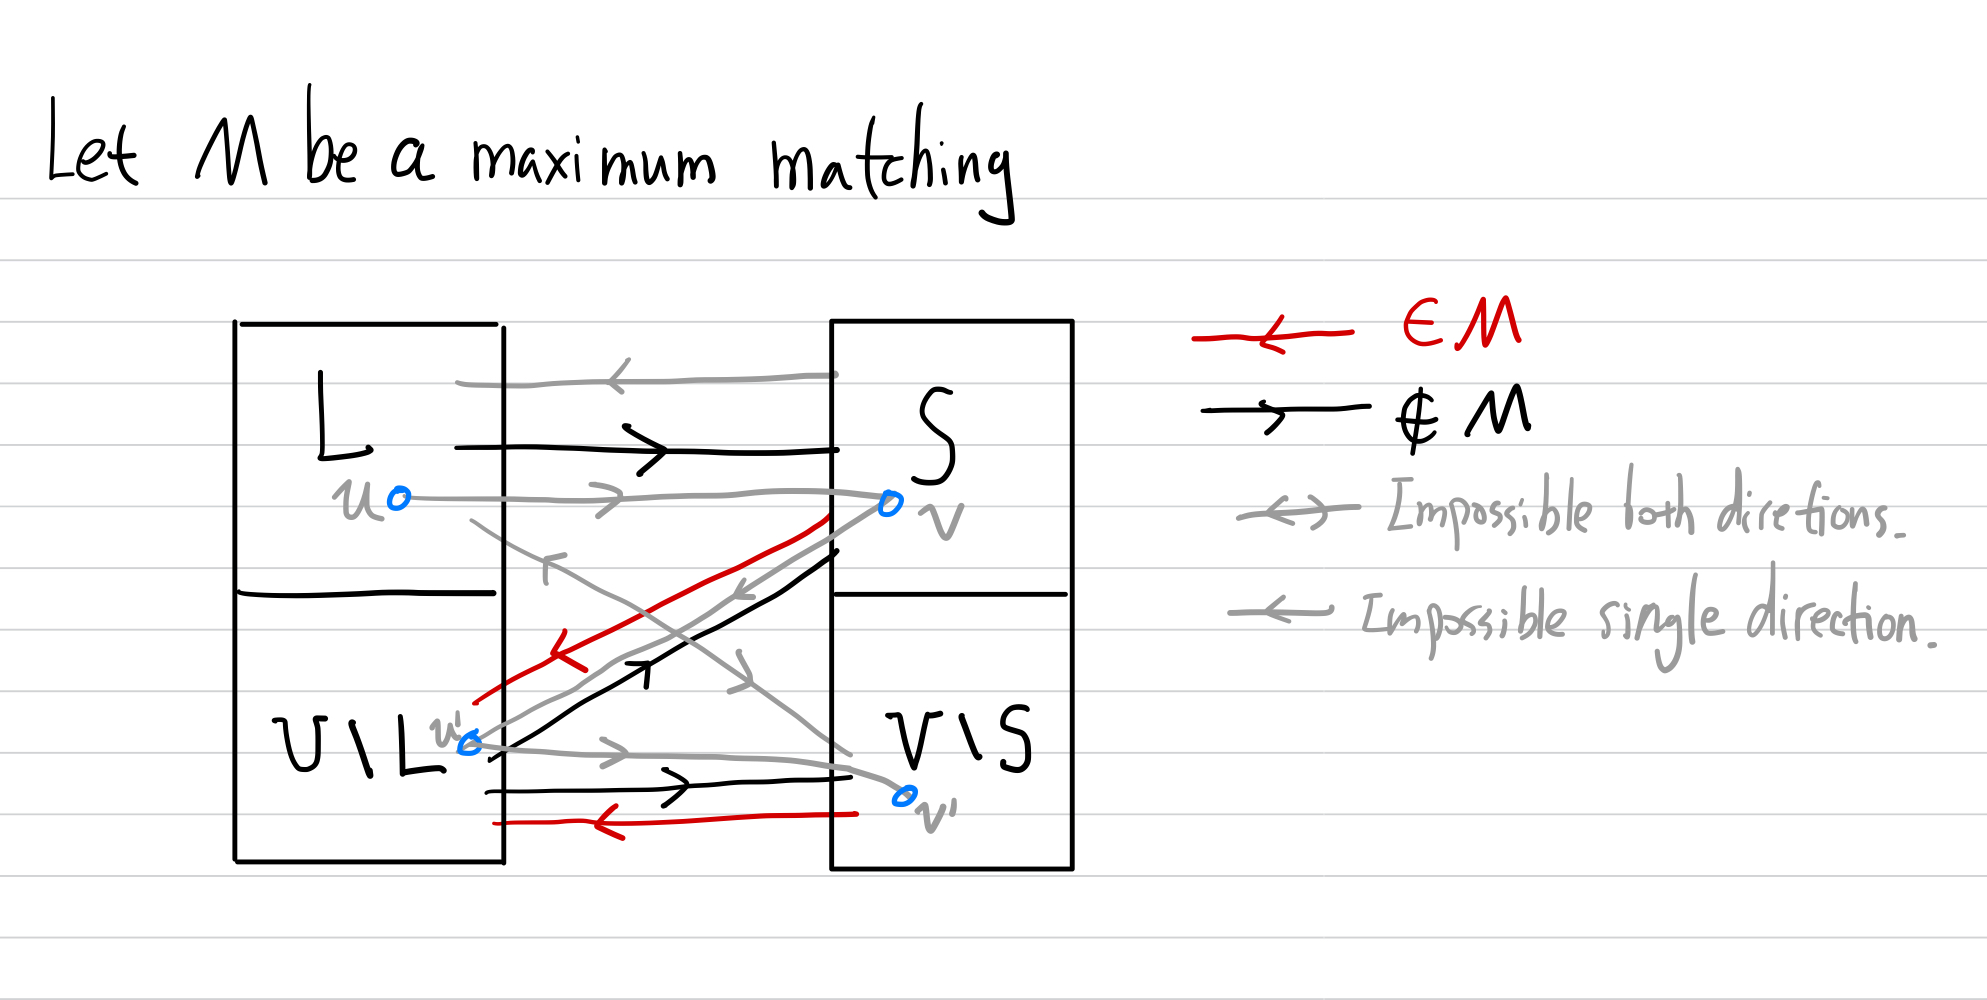
\includegraphics[width=12cm]{fig1.jpeg}
        \end{figure}
    \end{proof}

\section{Problem 3.25}
    \begin{theorem}
        Let $G =(V, E)$ be a bipartite graph. Then the perfect matching polytope $P$ is equal to the set of verctors $x\in \mathbb R^{|E|}$ satisfying: 
        \begin{align}\label{definition:Q}
            Q:= 
            \begin{cases}
                x_e \ge 0 \quad \forall e \in E
                \\
                \sum_{e\ni v}^{}x_e = 1\quad \forall v \in V    
            \end{cases}
        \end{align}
        Here let $G = (V\dot\cup U, E)$ be a bipartite graph and we denote $P$ as the polytope that is the convex hull of all possible perfect matching solution vectors. 
        \par
        Assuming that $|V| = |U| = n$ so that perfect matching is at least possible, notice that the perfect matching vector is a solution to the perfect matching problem we denote it as $\chi_M\in \mathbb \{0, 1\}^{|E|}$: 
        \begin{align}
            & \forall e\in E: (\chi_M)_e := 
            \begin{cases}
                1 & e \in M
                \\
                0 & \text{else}
            \end{cases}
            \\
            & P = \text{conv}\{\chi_M: M \text{ is a matching on G}\}
        \end{align}
        The theorem states that $P = Q$ \textbf{when} $G$ is bipartite. 
    \end{theorem}
    Observe that if $P = \emptyset$ then $Q = \emptyset$. This is obvious because if there is no perfect matching, then it's impossible to sum up all the edges incident to a vertex and sum up to 1. The trivial case holds up. 
    \subsection{Settings Things up}
        Let $G:= (U\dot\cup V, E)$ be bipartite, $w:\mathbb R^{|E|} \mapsto \mathbb R_+$ be a weight functions on all the edges of $G$. We further assum $|U|=|V| = n$, and the vertices are enumerable: 
        \begin{align}
            & U:= \{u_i\}_{i = 1}^n 
            \\
            & V:= \{v_i\}_{i= 1}^n 
        \end{align}
        Then we define another matrix $A\in \mathbb R^{n\times n}$, which represent the weight function $w$ for each edges on the bipartite graph: 
        \begin{align}
            a_{i, j} := \begin{cases}
                w(\{u_i, v_j\}) & \{u_i, v_j\} \in E
                \\
                0 & \text{else}
            \end{cases}
        \end{align}
    \subsection{Show $Q \subseteq P$}
        Take any $x\in Q$, then $x\in \mathbb R^{|E|}$, and it can define a weight function for all the edges on $E$: 
        \begin{align}
            w(e):= x_e
        \end{align}
        Which induces a matrix because assuming that $G$ is bipartite: 
        \begin{align}
            a_{i, j} := 
            \begin{cases}
                x_e & e=\{u_i, v_j\}, e\in E
                \\
                0 & \text{else}
            \end{cases}
        \end{align}
        For how $Q$ is defined in (\hyperref[definition:Q]{\ref*{definition:Q}}) we have this: 
        \begin{align}
            & \forall v \in U \dot\cup V:
            \sum_{v \ni e}^{}x_e = 1\quad x_e \ge 0 \; \forall e\in E
            \\
            \implies &
            \forall u_i \in U: \sum_{\{u_i, v_j\}\in E}^{} x_{\{u_i, v_j\}} = 1 = \sum_{j = 1}^{n} a_{i, j}
            \\
            \implies & 
            \forall v_j \in V: \sum_{\{u_i, v_j\}\in E}^{} x_{\{u_i, v_j\}} = 1 = \sum_{i = 1}^{n} a_{i, j}
        \end{align}
        For any vertices in $G$, we can break it into 2 cases, in $U$ or $V$. For both cases we can invoke the definition of $Q$, and sume up all $x_e$ where $e$ is incident to the vertex: $u_i, v_j$. Then by the definition of $a_{i, j}$ back in (2.2.2), both of them has to be equal to 1. Therefore, the matrix $A$ whose $(i, j)$ entry are $a_{i, j}$ are going to be a doubly stochastic matrix. The non-negativity constraint of $x_e$ translate to corresponding $a_{i, j}$ by (2.2.2) as well. 
        \par
        From 3.11 of the last HW, we know that the matrix $A$ is a convex combinations of permutations matrices. And most importantly, a permutation matrix is a perfect matching on a bipartite graph of the same size. Let $\mathbf P$ denotes any $n\times n$ permutations matrix, and let $\pi:[n]\mapsto [n]$ be bijective, then $\pi$ induces a permutations matrix: 
        \begin{align}
            \mathbf P := \begin{bmatrix}
                e_{\pi(1)} & e_{\pi(2)} & \cdots & e_{\pi(n)}
            \end{bmatrix}
            \\
            \text{define }\mathcal M_{\mathbf P} \text{ s.t: }
            \mathbf P_{i, j} \neq 0 \iff 
            \{u_i, u_j\} \in \mathcal M_{\mathbf P}
            \\
            \implies \mathcal M_{\mathbf P} \text{ is a matching on G}
        \end{align}
        This is true because for each $v_j\in V$, $\exists! \{u_{\pi(j)}, v_j\} \in \mathcal M_{\mathbf P}$. Therefore all vertices in $U$ are covered, and since $|U|=|V|=n$, the matching is perfect. Further more, the matching introduced by $\mathbf P$ can be converted into a binary vector in $\chi_{\mathcal M_{\mathbf P}}\in \{1, 0\}^{|E|}$: 
        \begin{align}
            (\chi_{\mathcal M_{\mathbf P}})_e = 1 \iff e\in \mathcal M_{\mathbf P}
        \end{align}
        For each non zero element $a_{i, j}$, they are a convex combinations of all possible $\mathbf P_{i, j}$ where $\mathbf P$ is a permutation matrix, by (2.2.2) we know that $x_e$ is a convex combinations of all possible $(\chi_{\mathcal M_{\mathbf P}})_e$. Therefore the whole vector $x$ is a convex combinations of $\chi_{\mathcal M_{\mathbf P}}$ for all possible $\mathbf P$;  $x$ now fits the definition of $P$, therefore, $Q\subseteq P$. 
    \subsection{Show $P\subseteq Q$}
        This is true because each $\chi_{M}$ is also an element of $Q$, this is direct from the definition of a perfect matching (we don't even need $G$ to be bipartite in this direction). Using the fact that the set $Q$ is convex, and it contains all $\chi_{M}$, therefore, it contains the convex hull of all $\chi_{M}$.
    \begin{proof}[Theorem 1]
        Since $P\subseteq Q$ and $Q\subseteq P$ from the previous 2 sections, $P=Q$. 
    \end{proof} 
    
\section{Problem 8.4}
    Let $G = (V, E)$ be a graph. Describe the problem of finding a clique (= complete subgraph) of maximum cardinality as an integer linear programming problem. 
    \par
    We consider decision variables of both vertices and edges. Let $x\in [0, 1]^{|V|}$, then: 
    \begin{align}
        P & := \forall {u, v}\not \in E: 
                x_u + x_v \le 1
        \\
        P_I &:= P \cap \mathbb Z^{|E| + |V|} \leftarrow \text{This is what we want}
    \end{align}
    For every vertices chosen, there must exist an edge $e\in E$ between them, then it will be a clique on the graph. To assert it we prevent the case where $u, v$ are chosen and there is no edges betwee them (which is (2.0.1)). The second line (2.0.2) asserts the conditions that we want the integral solutions. 

\section{Problem 8.7}
    \begin{prop}
        Give integer matrix $A$ and an integer vector $b$ s.t: polyhedron $P:= \{x|Ax \le b\}$ is integer and $A$ is not T.U (totally Unimodular). 
    \end{prop}
    \par
    For the trivial case consider $A\in \mathbb R^{1\times 1}$, $A = 2$, and the polytope: $P:=\{x|Ax \le 4\}$, then: 
    \begin{align}
        2x \le 4 \implies x = 2
    \end{align}
    The vertex is an integer and $\det(A) = 2$, not T.U. For a bigger example consider: 
    \begin{align}
        A := \begin{bmatrix}
            2 & 0
            \\
            0 & 2
            \\
            -1 & 0
            \\
            0 & -1
        \end{bmatrix}
        b := \begin{bmatrix}
            2 \\2 \\ 0\\ 0
        \end{bmatrix}
    \end{align}
    Then determinant of upper 2 by 2 of $A$ is not $4$ which means $A$ is not T.U. Next the polytope define by such $A, b$ will heve vertex: $[0\; 1]^T, [1\; 0]^T$ which are integral. 


\end{document}